\documentclass{article}
\usepackage[utf8]{inputenc}
\usepackage{amsmath}
\usepackage{amssymb}
\usepackage{hyperref}
\usepackage{graphicx}
\graphicspath{ {Images/} }

\hypersetup{
    colorlinks=true,
    linkcolor=blue,
    filecolor=magenta,      
    urlcolor=cyan,
}

\urlstyle{same}

\title{Simplified Perishable Product Flow}
\author{dip7777}
\date{November 2017}

\begin{document}

\maketitle

\section{Objective Function}

We have the following simplified Objective Function for G = [N,L] where N is the set of Nodes and L is the set of Links with known demands $d_k$ at each of the $n_R$ endpoints:
$$Minimize \hspace{5mm} \sum_{a \in L}\hat{c}_a(f_a) + \sum_{k=1}^{n_R}(\lambda_k^-(d_k - \sum_{a \in IN_k}f_a) + \lambda_k^+(\sum_{a \in IN_k}f_a - d_k)) $$
subject to
\begin{align}
    f_a \geq 0 \hspace{10mm} \forall a \in L\\
    \sum_{a \in IN_n}f_a = \sum_{a \in OUT_n} f_a \hspace{2mm} \forall n \in N \hspace{2mm} except \hspace{2mm} at \hspace{2mm} origin \hspace{2mm} node \hspace{2mm} 1 \hspace{2mm} and \hspace{2mm} sinks
\end{align}

As discussed in the last meeting, our viewpoint is that $\hat{c}_a$ (the cost of transporting $f_a$ units of flow on link $a$) would be our objective function while the other two terms with $\lambda_k^-$ and $\lambda_k^+$ can be viewed as constraints (some kind of soft constraints) and have to be tried to be shifted outside the objective function to the `subject to' part. What we need is some kind of formulation with `link flows' (not path flows) whose dual leads to some kind of a cut. \break
To that end, we tried to reformulate the second part of the objective function with the shortage-surplus to $\sum_{k=1}^{n_R}(d_k - \sum_{a \in IN_k}f_a)(\lambda_k^- - \lambda_k^+)$ \break \break
But the issue is that we need the $\lambda_k^-$ term  to kick in only when there is a shortage and $\lambda_k^+$ term to kick in only when there is a surplus. In the paper, they integrate between proper limits and hence it is taken care of.

\section{Attempted Reformulation}
\break
$$Minimize \hspace{5mm} \sum_{a \in L}\hat{c}_a(f_a) + \sum_{k=1}^{n_R}(\lambda_k^-short_k + \lambda_k^+excess_k) $$
subject to
\begin{align}
    f_a \geq 0 \hspace{10mm} \forall a \in L\\
    \sum_{a \in IN_n}f_a = \sum_{a \in OUT_n} f_a \hspace{2mm} \forall n \in N \hspace{2mm} except \hspace{2mm} at \hspace{2mm} origin \hspace{2mm} node \hspace{2mm} 1 \hspace{2mm} and \hspace{2mm} sinks\\
    short_k = (1 - q_{ks})(d_k - \sum_{a \in IN_k}f_a) \hspace{10mm} \forall k \hspace{2mm} in \hspace{2mm} set \hspace{2mm} of \hspace{2mm} sinks\\
    excess_k = (1 - q_{ke})(\sum_{a \in IN_k}f_a - d_k) \hspace{10mm} \forall k \hspace{2mm} in \hspace{2mm} set \hspace{2mm} of \hspace{2mm} sinks\\
    q_{ks} + q_{ke} \leq 1 \hspace{10mm} \forall k \hspace{2mm} in \hspace{2mm} set \hspace{2mm} of \hspace{2mm} sinks\\
    q_{ks}, q_{ke} \in \{0,1\} \hspace{10mm} \forall k \hspace{2mm} in \hspace{2mm} set \hspace{2mm} of \hspace{2mm} sinks
\end{align}

\section{Last week's work}
My task was set up a baseline and try to map our problem to the framework given in the paper \href{https://dslpitt.org/uai/papers/13/p459-nagano.pdf}{Structured Convex Optimization under Submodular Constraints SCOSC.} The \href{https://github.com/Ras-al-Ghul/Perishable-Flow-Optimization/tree/master/Codes}{baseline} has been setup (refer diagram below). Please go through it once to check for correctness and also to gain familiarity with the constrains through the comments in the PerishableFlow.mod file.
\break
\break
At first, while reading the SCOSC paper, it seemed that they only considered capacities or costs - not both because the examples were all about Minimizing some cut (which in turn means maximizing the flow) - which is definitely not directly applicable to our problem. But I think the title 'Convex Optimization under Submodular Constraints' means that the cost function (edge costs) in our problem is the 'Convex Optimization' part while the cut defined over capacities in our problem is the 'Submodular Constraints' part. So we should be able to map it.
\break
\break
Let us consider problem (1.a) from the SCOSC paper and the PerishableFlow.mod (PF.mod) file. The $x_i$'s ($x_i^2$'s) in (1.a) correspond to the $f[i]$'s from the PF.mod file - a 1D vector. The $b_i$'s from (1.a) correspond to $cost[i]$'s from PF.mod file - they will be a 1D vector. Now we have to see what $B(f)$ means. $f$ from the $B(f)$ would be the cut function associated with the capacities in our problem - we have only three real capacities - $d1, d2, d3$ The rest can all be given the same arbitrary high number as capacities (say for instance $d1+d2+d3$) $f$ would then be the $\sum$ defined over the capacities which form a part of the cut.
\break
\break
Let us now look at the constraints. The flow constraints from our problem hold as usual - I think this is already considered in the SCOSC paper. Same is true for the flow positive constraints - i.e. $flow \hspace{1mm} is >= 0$ over all the edges. Coming to the $initflow: (f[1] + f[2]) <= (d1 + d2 + d3)$ constraint from the PF.mod file, this will hold in the SCOSC setup without adding anything because the capacities on the three new edges to the super-sink will take care of it. (Now this is assuming $flows \hspace{1mm} on \hspace{1mm} all \hspace{1mm} edges >= 0$ holds) (Please look into this as I may be wrong here with this assumption and reasoning)
\break
\break
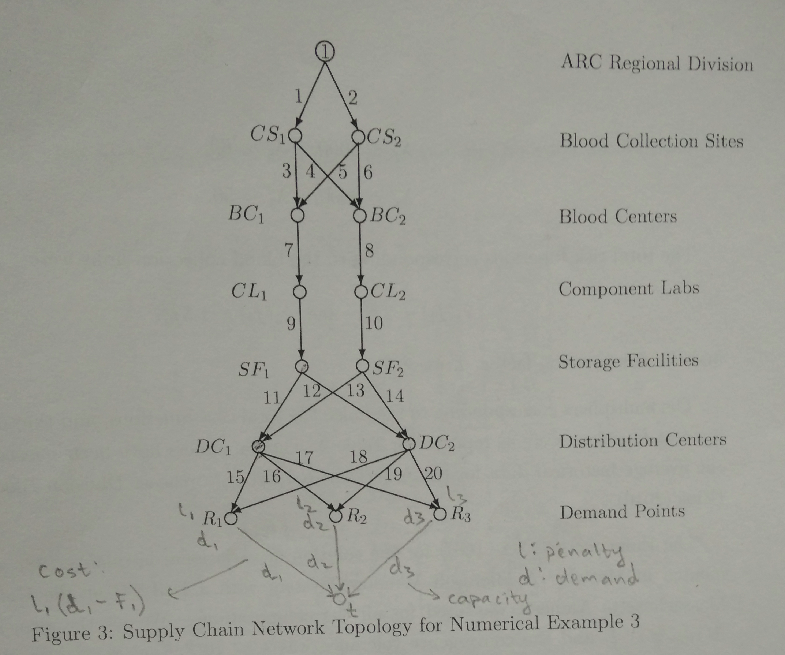
\includegraphics[width=14cm, height=14cm]{Diagram}
\break
Now the important thing that is left is how to handle cost on the three new edges to the supersink - i.e. how to map it to the SCOSC paper's framework. As I see it, there might be two ways to go about this (I think Prof. Praveen maybe able to help here). 
\break
\break
One way is as follows: look at the cost $l1 \times (d1 - f1)$. On every link, we have cost associated with flow. On this link, we have cost associated with lack of flow. So we could try to map it to one of the equivalent forms (1.a) - (1.f) maybe (1.e) is the closest. Don't know if we will be able to map it exactly. Also more importantly, can we combine objectives of different forms? (because rest of the edge costs will be of the (1.a) form)
\break
\break
The other way is as follows: make the cost $- (l1 \times f1)$ In this way, it will fit into (1.a) form of the SCOSC paper. The max flow will be taken care of by the capacity constraint. We're ensuring that every unit of flow within $d1$ is being rewarded in terms of reducing the optimization function further. This is definitely optimal if we solve unit flows at a time over iterations - I'm not sure if it will give the optimal solution if we directly plug it into the SCOSC framework.

\section{Submodular Flow Problem}
Now that was regarding last week's work. Since we may not be looking at distributed approaches anymore, I think Submodular Flow Problem might also be a relevant fit here. Please see Page 280 from \href{https://github.com/Ras-al-Ghul/Perishable-Flow-Optimization/blob/master/Papers/Submodular-Functions-and-Optimization.pdf}{this book.} A Neoflow Problem with a Separable Convex Cost Function. (book title in case the link doesn't work - Submodular Functions and Optimization - from the Github repo/papers) This has 'separable' in it and deals with convex cost functions - the author suggests an out-of-kilter kind of method - is this relevant here? Can this be decentralized?

\section{Distributed Methods}
I was looking at keywords like 'distributed submodular`, `decentralized submodular`, `distributed network simplex` and came across this paper \href{http://www.rle.mit.edu/ncrc/wp-content/uploads/2014/02/2005_achieving.pdf}{Achieving Minimum Cost Multicast - A decentralized approach based on network coding} They have a very very similar objective function and a decentralized approach - is this better than looking for submodularity?


\end{document}

